%\addbibresource{/home/jorgsk/phdproject/bibtex/jorgsk.bib}

%What results should you present? Anything more than was presented in the paper?

%The figure with the compartments and poly(A)-.

%Shows two things: 1) there is poly(A) signal in poly(A)- extract. explained by
%errors in screening and possibly by short poly(A). 2) intronic polyadenylation in the nucleus overrepresented. Makes
%sense if there is nuclear degradation of intronic poly(A) which has been
%recently shown.

%Then the figure with overlap to show how much you get?

%Then the figure that shows the flattening out of the getting of new
%transcripts.

%Discuss each of the tree figures and that's it.

%Maybe make a table with some of the numbers from the statistics you output.

We developed a software called Utail and ran it on the ENCODE RNA-seq data to
characterize polyadenylation sites in 12 human cell lines. Parts of the
analysis was published in Nature by Djabeli et al. First we summarize the
findings in the Djabeli et al study before we go on to adress the findings that
were not included in the paper.

\subsection{The ENCODE pilot project}
After the complete human genome was published in 2003, the ENCODE pilot project
was launched to investigate in detail 1\% of the human genome through a
collaboration of research labs all over the world. With the then prevalent genome-wide
technologies, which included among others microarrays, CAGE, and ChIP-Chip,
combined with bioinformatic analysis, the outcome was a wealth of data that
confirmed previous tentative genome-wide findings, added new knowledge, and was
used to improve the annotation the human genome. The outcome was published in a
group paper in Nature \cite{birney_identification_2007} as well as in 28
companion papers in a special edition of Genome Research. The data generated
is freely available from http://genome.ucsc.edu/ENCODE/ including important
metadata about how the experiments were performed.

\subsection{The ENCODE follow-up project}
The ENCODE pilot was deemed a success and led to a follow-up project that would
cover 100\% of the genome. This was made possible by the then-emerging
next-generation DNA sequencing technology which had considerably lowered the
cost of sequencing while also increasing the throughput. Now the technologies
from the ENCODE pilot were taken to the next level: microarrays were generally
substituted for RNA-seq, CAGE could use next-gen sequencers instead of Sanger
sequencing, and ChIP-Chip was replaced by ChIP-seq.

As of mid 2012 the follow-up ENCODE papers are in the process of being
published. A summary paper has been published / accepted. A paper focusing
mostly on the transcriptome has been published in XXX and it is to this paper
that we have made a contribution. This is the hitherto largest genome-wide
investigation of the width and breath of transcription in human cells.

The paper by Djabeli et al. finds that the cumulative coverage for 15 human
cell lines is 62\% for processed transcripts and 75\% for primary transcripts.
In other words, three quarters of the human genome is transcribed. However, the
average coverage for each cell line was 22\% and 39\% for processed and primary
transcripts. This tells us that while most of the genome is capable of being
transcribed, each cell will express little more than a quarter of it. They
discovered by using the Cufflinks software 45\% more transcripts than is
currently annotated, with most of the newly identified transcripts landing in
intergenic regions. The consequence is that the intergenic regions decreased in
median length from around 14.000 to 4.000, showing that the human genome is not
as "barren" as was once thought. They found 22.000 new splice sites,
demonstrating the flexibility of the human genome whereby each gene may express
multiple RNA isoforms. Even though many genes were found to express up to 12
alternative isoforms, 30\% of protein coding genes expressed a dominant isoform
and three quarters had two or more dominant isoforms. This shows that while
alternative isoform usage is ubiquitous, mostly one or two isoforms will be
used per gene. In other words, while the one-gene one-protein model is not
correct in humans, it is often a decent approximation. Additionally, they
discovered many new long noncoding RNAs (lncRNA). These RNA appear similar to
mRNA and undergo processing, but do not code for protein. An over-all
conclusion is that protein coding transcripts are highly expressed, while
non-coding transcripts like lncRNA are generally lowly expressed, down to less
than one transcript estimated per cell. Using PET-data, they discovered roughly
128.000 transcription start sites (TTS), of which around 30.000 were novel.
They also discovered around 129.000 cleavage and polyadenylation sites inside
annotated transcripts, 80\% of which were not previously annotated. This shows
that transcription start sites are generally better annotated than
transcription termination sites.


\subsection{The dataset}
The datasets used in this study were generated by the ENCODE
(\textbf{Enc}yclopedia \textbf{O}f \textbf{D}NA \textbf{E}lements) consortium
and are available from http://hgdownload-test.cse.ucsc.edu/goldenPath/hg19/encodeDCC/wgEncodeCshlLongRnaSeq/

The data was generated from RNA-seq experiments from 12 human cell lines. Six
of the cell lines have RNA-seq data from whole cell extracts and the remaining
six cell lines have RNA-seq data from cytoplasmic and nuclear extracts in
addition to whole cell extracts. Each cell line is further available in both the
poly(A)+ and poly(A)- fractions of the RNA pool. Table \ref{tab:Datasets} shows
the cell lines and compartments used; as can be seen, most experiments were
available with a biological replicate. In total, 23 datasets were from whole
cell extracts, 11 were from cytoplasmic extracts, and 12 were from nuclear
extracts. This brings the total to 92 RNA-seq datasets. The datasets contains
only RNA-seq from long RNA, defined as RNA over 200 nucleotides in length. Each
dataset has been generated with Illumina paired-ended sequencing with a
read-length of 75 basepairs. Each dataset contains between 150 and 250 million
reads.

\begin{table}
	\centering
	\begin{tabular}{cccc}
	  Cell line & Whole Cell & Cytoplasm & Nucleus \\
	  \midrule
	  GM12878 & 2 & 2 & 2 \\
	  K562 & 2 & 2 & 2 \\
	  HeLa-S3 & 2 & 2 & 2 \\
	  HUVEC & 2 & 2 & 2 \\
	  HEPG2 & 2 & 2 & 2 \\
	  H1Hesc & 1 & 1 & 1 \\
	  Nhek & 2 & 0 & 1 \\
	  MCF7 & 2 & 0 & 0 \\
	  AG04450 & 2 & 0 & 0 \\
	  HSMM & 2 & 0 & 0 \\
	  NHLF & 2 & 0 & 0 \\
	  A549 & 2 & 0 & 0 \\
	\end{tabular}
	\caption{Number of replicates of the datasets from the ENCODE consortium}
	\label{tab:Datasets}
\end{table}

What sets this library apart from most RNA-seq data is that the cell is
compartmentalized and that both the poly(A)+ and poly(A)- fractions of RNA have
been sequenced separately. As mentioned in the introduction, the poly(A)+
fraction of an RNA sample contains all the RNA that is captured by a poly(T)
primer. This will include all processed mRNA with a poly(A) tail of more than
20 nucleotides (the length of the poly(T) primer). The poly(A)- fraction is the
complement of the poly(A)+ fraction and contains mostly noncoding RNA and
pre-processed mRNA.

The extra dimensions introduced by compartmentalizing the RNA pool and further
dividing it into poly(A)+ and poly(A)- fractions increase the resolution of the
data, allowing new questions to be asked. For example, it is now possible to
identify which transcripts are never transported to the cytoplasm. One could
also look at the poly(A)- fraction of transcripts in the cytoplasm to
distinguish between noncoding RNA in the nucleus and the cytoplasm on a
genome-wide scale.

\subsection{The short RNA mapper}
The short read mapper used in this work is the GEM mapper
\cite{ribeca_gem_2010}. The GEM mapper has been developed in the group of
Roderic Guigo and is production ready, although it has not been published yet.

\subsection{The PET data}
A high-throughput sequencing technique that is specific for locating the 3\p
end of transcripts is Paired End diTag (PET) Sequencing. This technique
adds two tags to the 3\p end and the 5\p end of an RNA. Those tags then join
with each other, forming a circular RNA. Subsequently, only the sequences close
to the two tags are sequenced. Thereby, one obtains the sequence information
about both the transcription start site and the transcript termination site of
the RNA. By mapping those sequences back to the genome, it is possible to find
out where the RNA began and ended. We have used PET data developed by ENCODE
which is available from
http://hgdownload.cse.ucsc.edu/goldenPath/hg19/encodeDCC/wgEncodeGisRnaPet/ to
compare with the polyadenylation sites we discovered. We demanded a coverage of
10 PET reads to accept a site as transcript termination site.

\section{Methods}
The description of the methods we used are found in the supplementary materials
of the paper by Djabeli et al. and in the section about Utail in the Appendix.
Briefly, the method involves mapping polyadenylation sites onto the genome and
clustering them if they are within 20 nucleotides of each other, since this is
close to the maximal range of the stochastic effect of choice of 3\p cleavage
site \cite{tian_large-scale_2005}. After clustering we search the genomic
sequence 40 nucleotides downstream the polyadenylation site for one of the
polyadenylation signals (PAS). Finally we intersect the polyadenylation sites
with the 3\p PET sites and annotated poly(A) sites to see which overlap.

\section{Results}
<<<<<<< HEAD
We developed a software called Utail and ran it on the ENCODE RNA-seq data.
For details on how Utail works, see the Appendix. Parts of the analysis from
Utail's output was published in Djabeli et al. XXX. Here we describe the parts
of the analysis that was not included in paper.

\section{Methods}
The description of the methods we used are found in the supplementary materials
of the paper by Djabeli et al. and in the Appendix. Briefly, the method
involves mapping polyadenylation sites onto the genome and clustering them if
they are within 20 nucleotides of each other, since this is close to the
maximal range of the stochastic effect of choice of 3\p cleavage site
\cite{tian_large-scale_2005}. After clustering we search the genomic sequence
40 nucleotides downstream the polyadenylation site for one of the
polyadenylation signals (PAS). Finally we intersect the polyadenylation sites
with the 3\p PET sites to see which overlap. To avoid false positives, we check
the genomic sequence for poly(A) tracts and discard putative poly(A) reads that
land at a genomic location that is poly(A) rich. Further we filter out poly(A)
reads that map to intron-exon junctions, since several false positives were
found at these locations.

Here we add the results that were not published in the Djabeli et al. study.

\subsection{Total number of polyadenylation sites}
By merging all polyadenylation sites from all datasets, we identified a total
of around 158.000 polyadenylation sites in the genome for the poly(A)+ fraction
and around 86000 polyadenylation sites for the poly(A)- fraction. Figure
\ref{fig:saturation} shows how the number of new polyadenylation sites
saturates as the number of datasets increases. The saturation is sharper for
polyadenylation sites which have are annotated with a downstream PAS. Since we
consider polyadenylation sites with a downstream PAS as more likely to be a
true positive, the different saturation curve for non-PAS and PAS-associated
polyadenylation sites is an indication that the number of false positives
increases when the number of clustered reads becomes very large. 

\subsection{Distribution of polyadenylation sites across the genome}
As expected, we found that most of the polyadenylation sites are in the 3\p UTR
exonic regions, but we located many polyadenylation sites in the intergenic
and intronic regions as well, see Figure \ref{fig:sidebars}. In the poly(A)+
fraction, there is more intronic poly(A) sites in the nucleus than in the
cytoplasm. This can partially be expected since most introns are removed in the
nucleus. Some introns, however, are included in the final mRNA (called intron
inclusion), and some introns are know to contain poly(A) sites
\cite{tian_widespread_2007}. 

We also found evidence for polyadenylated RNA in the poly(A)- fraction, see
Figure \ref{fig:sidebars} B. This was unexpected, since the poly(A)- fraction
is by design not supposed to contain RNA with poly(A) tails. We propose that
the polyadenylated RNA in the poly(A)- fraction have three possible sources.
The first source (S1) is purely technical: normal poly(A)+ mRNA with full
length poly(A) may not get adsorbed during the poly(A)+ filtration step and
thereby end up in the poly(A)- fraction. Source two (S2) and source three (S3)
are on the other hand of biological origin. S2 is mRNA with poly(A) tails that
are for some reason shorter than 20nt, which is the the threshold of the
poly(A)+ filtration step. One possibility is that they have had their polyA
tails degraded to below 20 nucleotides, which happens during mRNA degradation.
Another possibility is that they were actively undergoing polyadenylation at
the time of sampling and did not reach a poly(A) tail length of more than 20
nucleotides. Source three (S3) on the other hand are distinct from the other
two since these poly(A) tails do not originate from 3\p processing of pre-mRNA.
Instead, we propose that S3 are RNA with shorter, degradation-related transient
poly(A) tails which have been identified in the nucleus of mammalian cells
\cite{lemay_nuclear_2010}.

\subsection{Isolating polyadenylation sites unique to the poly(A)- and poly(A)+
fractions}
We wanted to separate the S3 from the S1 and S2 poly(A) sites. We did this by
recognizing that many of the S1 and S2 sites are likely to be present in both
the poly(A)- and the poly(A)+ fractions, since these sites really belong to
poly(A)+ transcripts that have accidentally ended up in the poly(A)- fraction.
Therefore, we filtered out all the poly(A) sites that intersected the poly(A)+
and poly(A)- fraction and removed these from both fractions. As can be seen in
in Figure \ref{fig:sidebars_intersect}, almost no poly(A) sites were found in
the pure poly(A)- fraction of the cytoplasm. The nuclear pure poly(A)- fraction
has fewer polyadenylation sites predominantly in the 3UTR exonic region, while
the number of sites in the intergenic and intronic regions did not change much.

\begin{figure}[htb]
	\begin{center}
		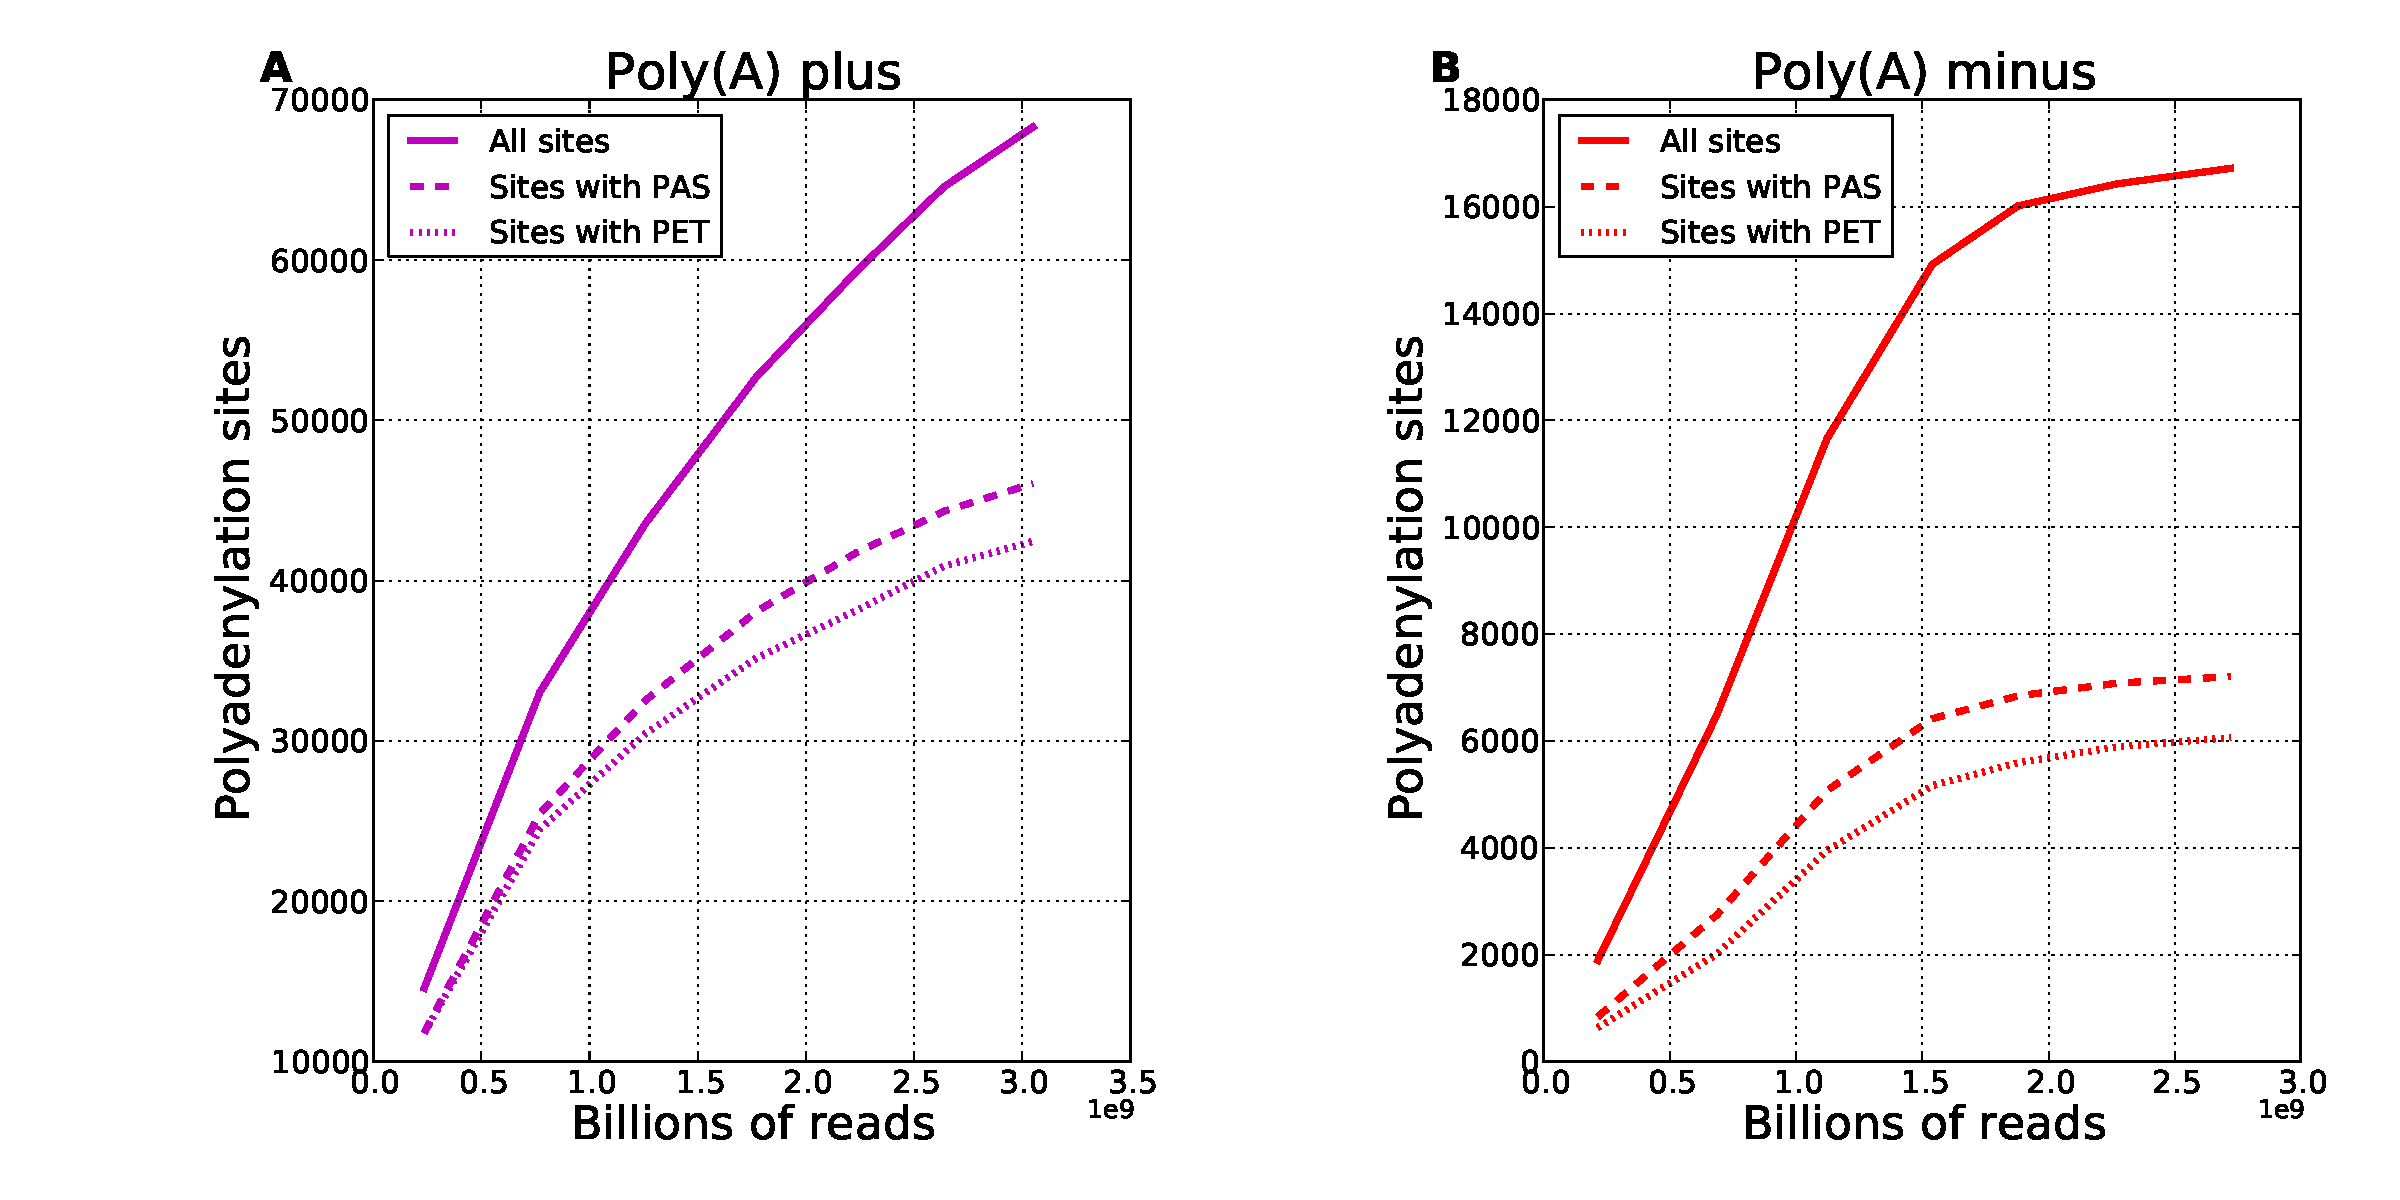
\includegraphics[scale=0.3]{figures/polyadenylation/Saturation_plot_2+.pdf}
	\end{center}
	\caption{Saturation of discovery of polyadenylation sites}
	\label{fig:saturation}
\end{figure}

\begin{figure}[htb]
	\begin{center}
		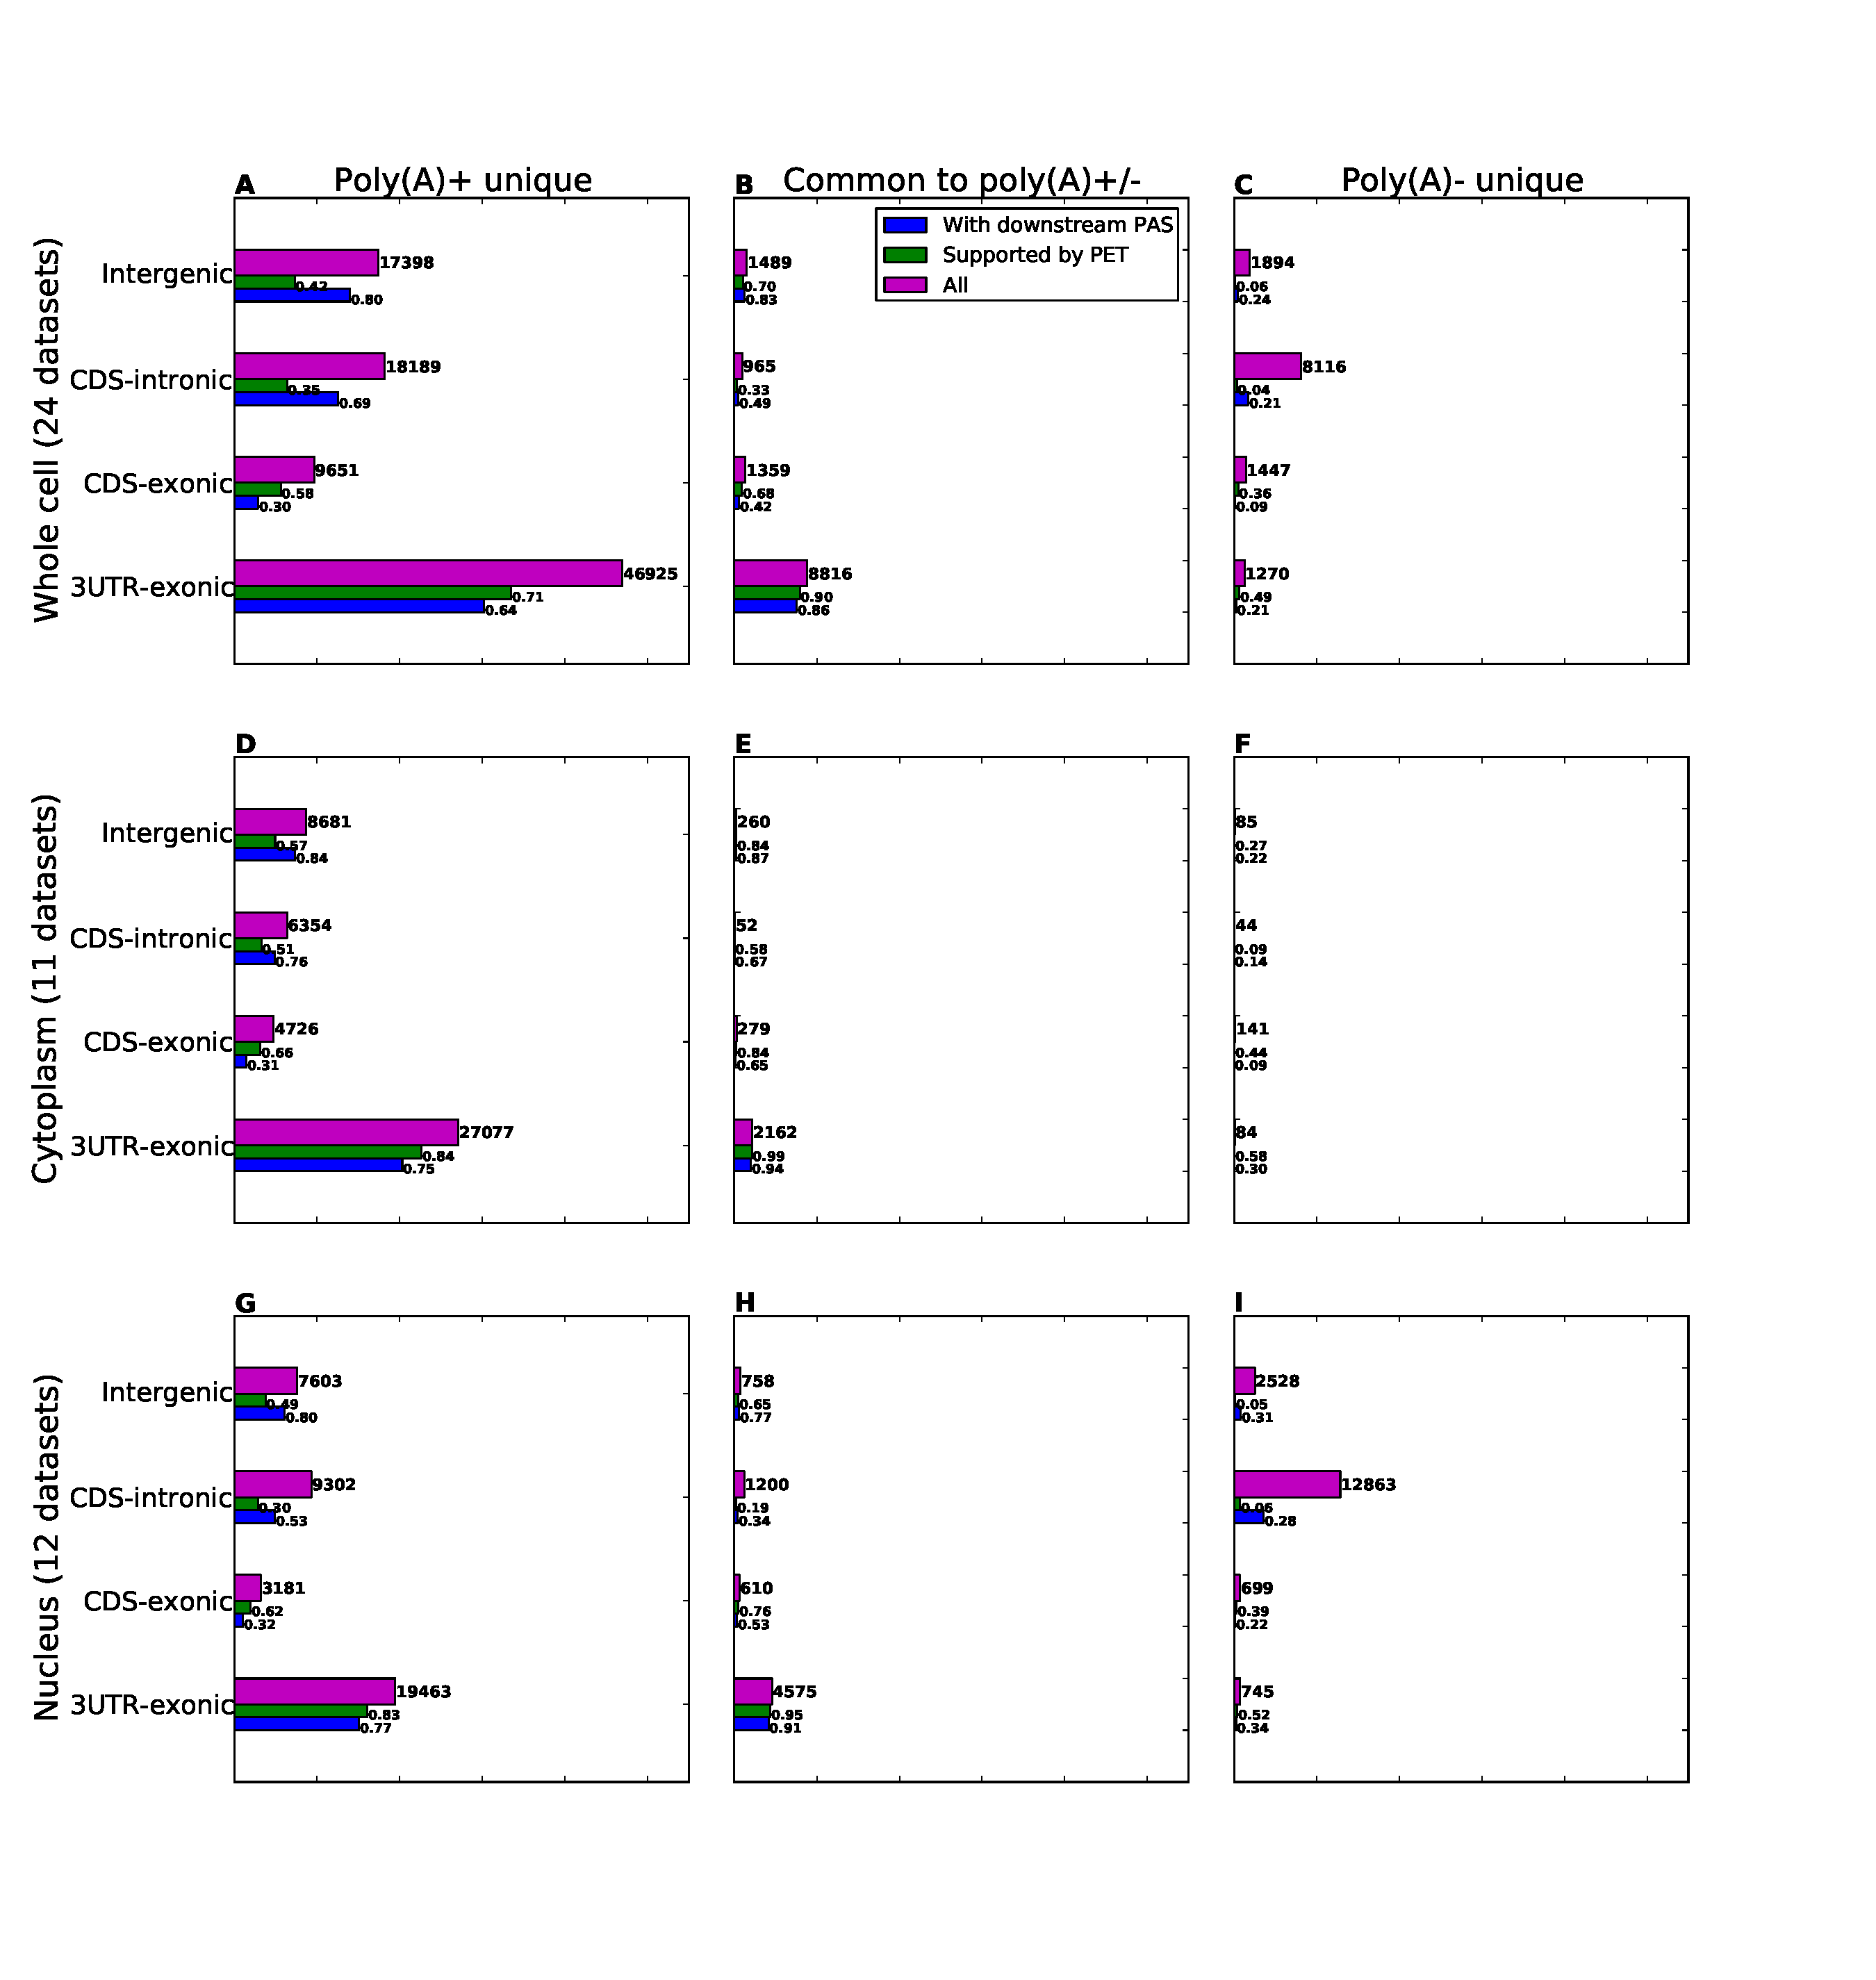
\includegraphics[scale=0.3]{figures/polyadenylation/intersected_sidebars_pA_2+.pdf}
	\end{center}
	\caption{Polyadenylation across genomic regions for the poly(A)+ and poly(A)-
	fractions and the sites that overlap the poly(A)+ and poly(A)- fractions}
	\label{fig:sidebars_intersect}
\end{figure}

\begin{figure}[htb]
	\begin{center}
		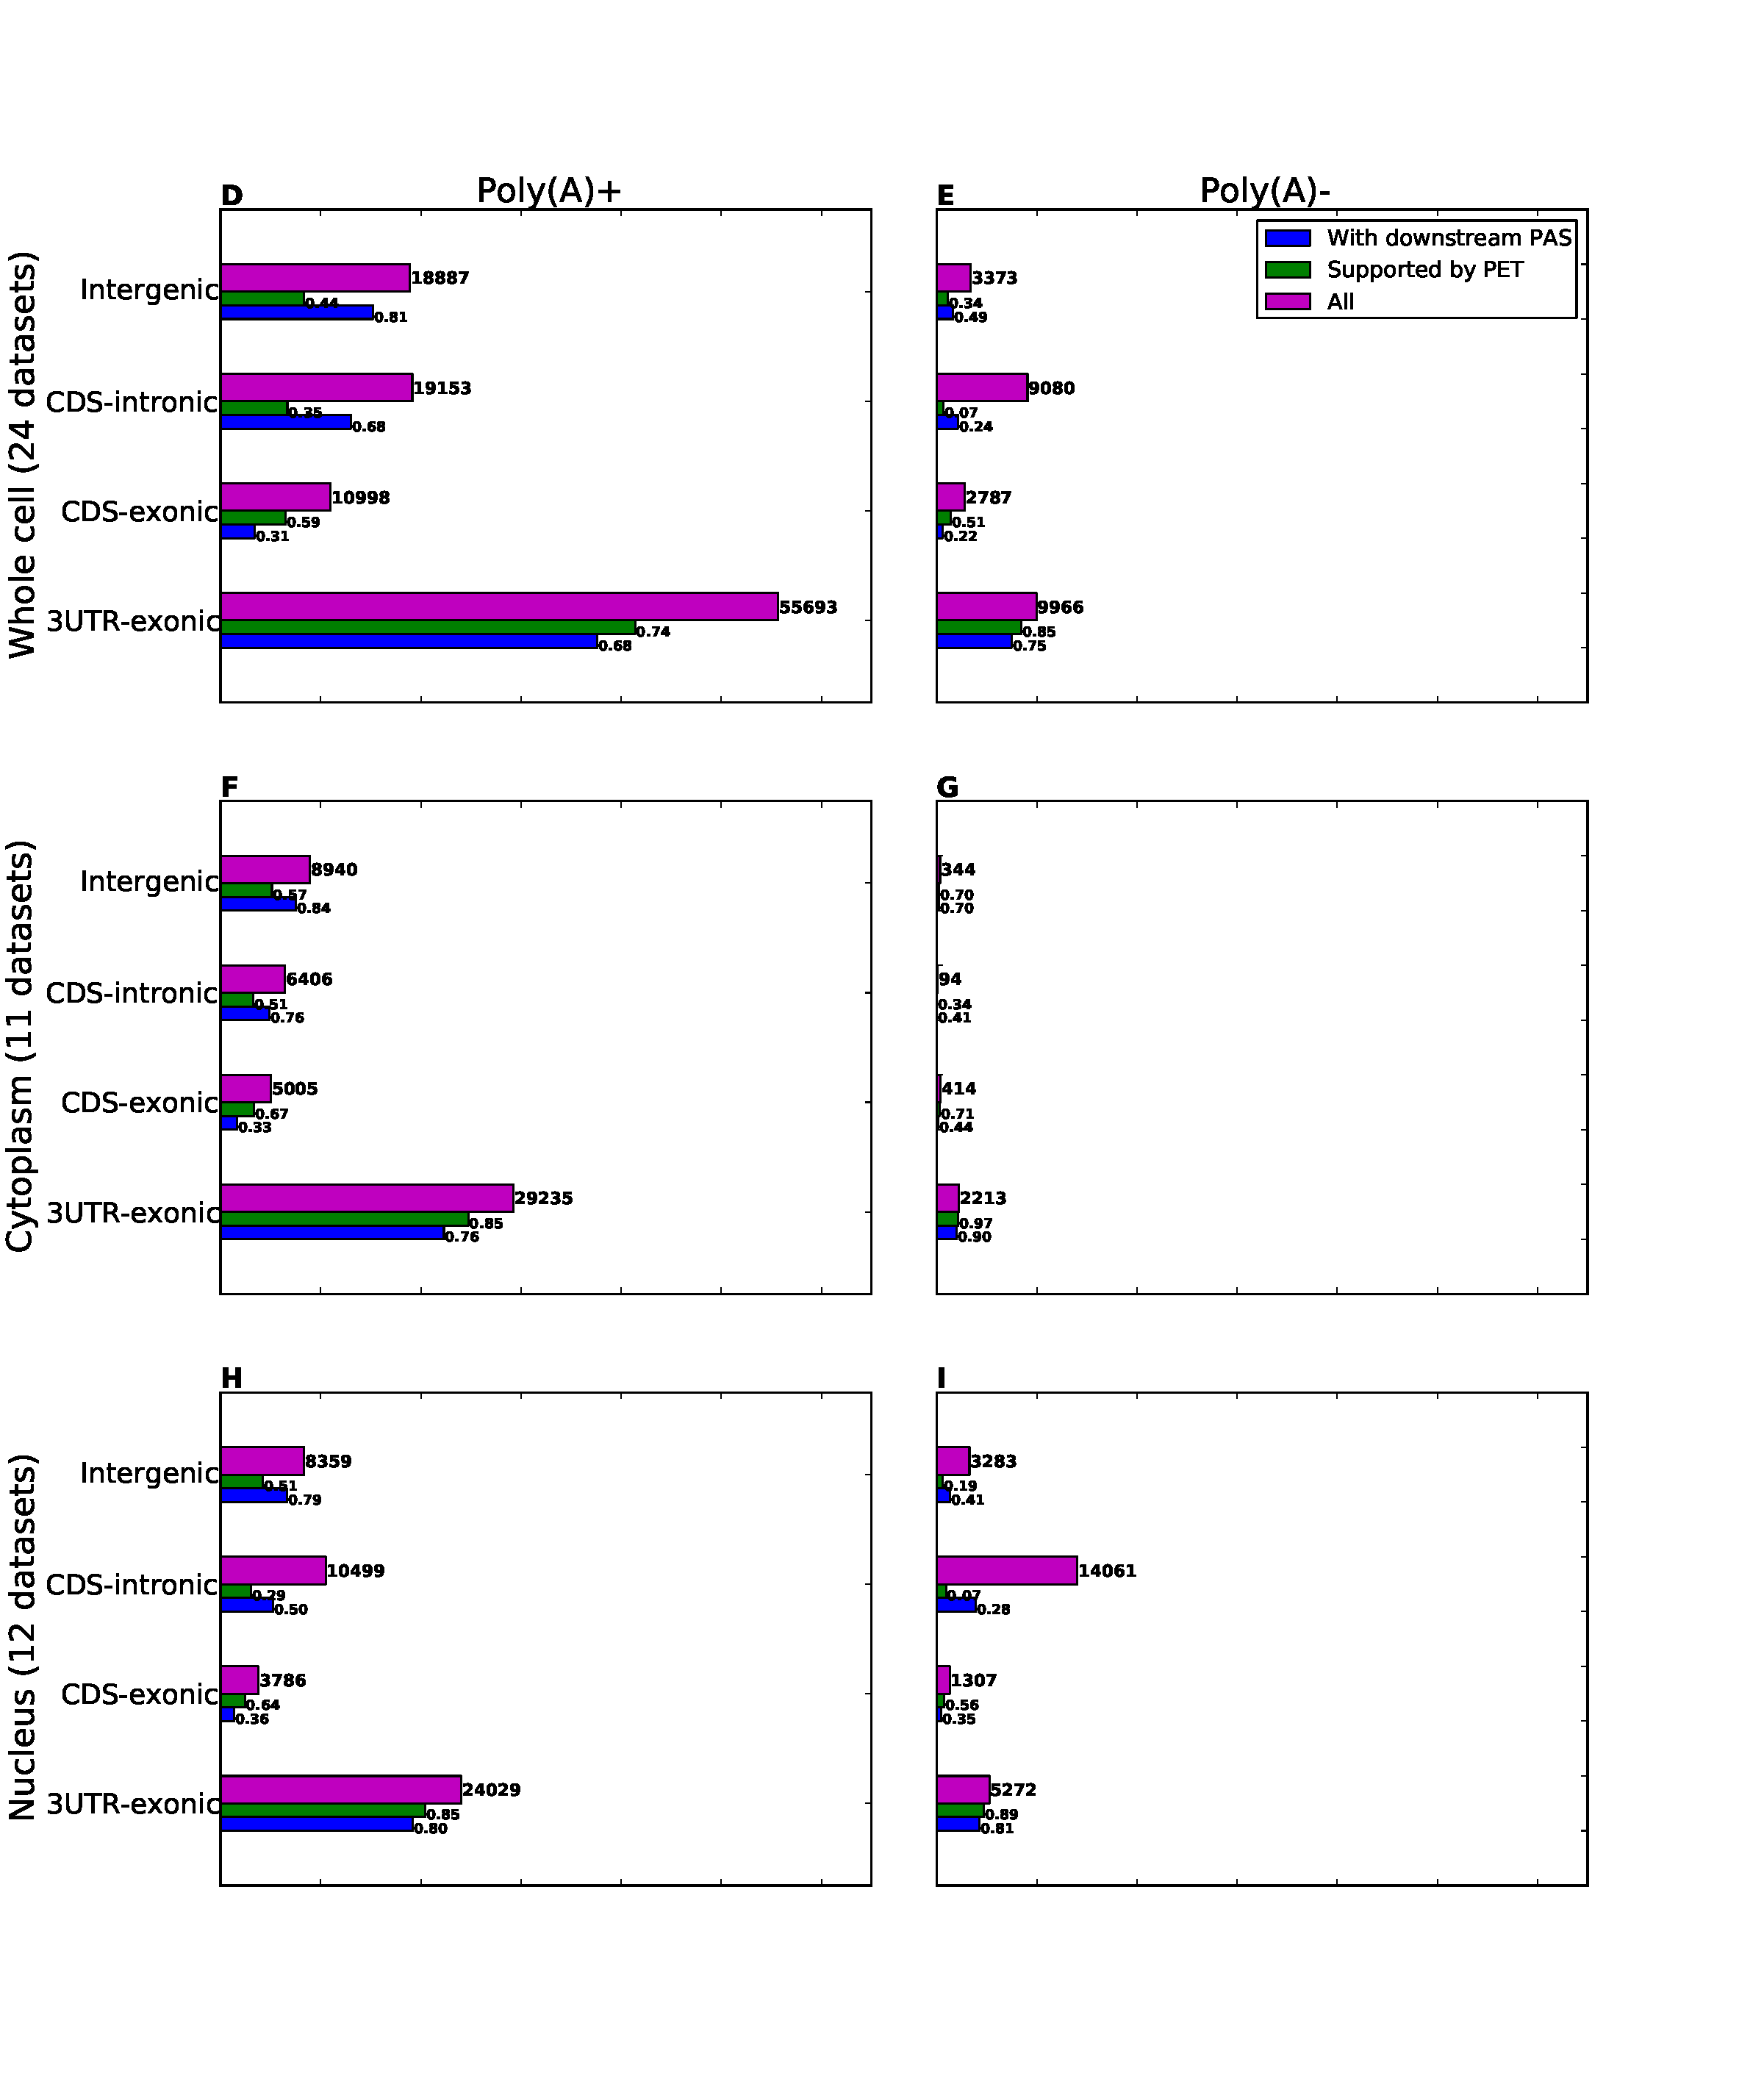
\includegraphics[scale=0.4]{figures/polyadenylation/Sidebars_pA_2+.pdf}
	\end{center}
	\caption{Polyadenylation across genomic regions for the poly(A)+ and poly(A)-
	fractions}
	\label{fig:sidebars}
\end{figure}

\subsubsection{Discussion}
By combining over 100 billion sequence fragments from 12 difference cell lines
in two different cell compartments in the poly(A)+ and poly(A)- fraction of
RNA, we have found over 150.000 polyadenylation sites in the transcriptome. Of
these sites, between \ldots XXX continue here!

The polyadenylation in intergenic regions indicate either unannotated long 3\p
UTR ends or cleavage and polyadenylation sites of novel transcripts.

We believe that the enrichment of the poly(A)- poly(A) sites in the nuclear
fraction in general is due to degradation-related transient polyadenylation
that occurs in the nucleus of mammalian cells \cite{lemay_nuclear_2010,
lacava_rna_2005, wyers_cryptic_2005}. In the nuclear compartment, the intronic
region stands out, but part of this is due to the fact that introns comprise a
large part of nuclear RNA, since human pre-mRNA sequences contain over 20 times
more intronic than exonic sequence \cite{venter_sequence_2001}. The low number
of poly(A) clusters in the cytoplasmic poly(A)- fraction is further an
indication that the number of false positive poly(A) sites is not very large.

TODO more discussion? More results? Alternative poly(A) or poly(A) in the
